\documentclass [tikz] {standalone}
\input{header.htex}

\begin {document}
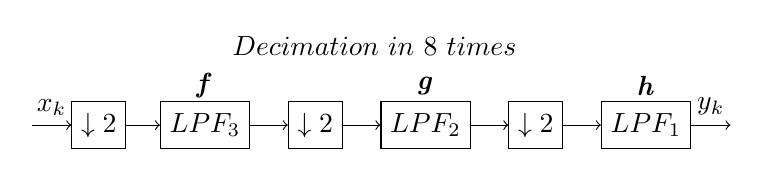
\begin{tikzpicture}

\node(title) at (3.5, 1) {$Decimation$ $in$ $8$ $times$};

\node(u0)[draw, minimum height=0.6cm] at (0, 0) {$\downarrow  2$};
\node(u1)[draw, minimum height=0.6cm] at (1.35, 0) {$LPF_3$};
\node(text1) at (1.35, 0.5) {\textbf{\emph{f}}};
\node(u2)[draw, minimum height=0.6cm] at (2.75, 0) {$\downarrow  2$};
\node(u3)[draw, minimum height=0.6cm] at (4.15, 0) {$LPF_2$};
\node(text1) at (4.15, 0.5) {\textbf{\emph{g}}};
\node(u4)[draw, minimum height=0.6cm] at (5.55, 0) {$\downarrow  2$};
\node(u5)[draw, minimum height=0.6cm] at (6.95, 0) {$LPF_1$};
\node(text1) at (6.95, 0.5) {\textbf{\emph{h}}};

\draw[->] (u0)--(u1);
\draw[->] (u1)--(u2);
\draw[->] (u2)--(u3);
\draw[->] (u3)--(u4);
\draw[->] (u4)--(u5);

\draw [<-](u0.west) -- ++(-0.5,0) 
    node[midway,above]{$x_{k}$};
\draw [->](u5.east) -- ++(0.5,0) 
    node[midway,above]{$y_{k}$};
\end{tikzpicture}
\end {document}